\chapter[Plaquette-MIDO]{Plaquette-MIDO\raisebox{.3\baselineskip}{\normalsize\footnotemark}}
\footnotetext{\url{https://github.com/Dauphine-MIDO/plaquette-MIDO}}

Ce projet a pour but d'implémenter un code générant un fichier PDF détaillant les différents enseignements du Master 1 MIAGE en apprentissage à partir de la base de données de Dauphine. La finalité est d'automatiser le lancement du code de sorte que quotidiennement le fichier PDF soit mis à jour et publié en ligne.

À mon arrivée, un code permettait déjà la génération du fichier PDF. Certains passages du code étaient cependant à revoir pour améliorer l'esthétique du fichier PDF. De plus, le code initial était très peu généralisé à d'autres utilisateurs et plusieurs changements étaient nécessaire pour qu'un autre utilisateur puisse lancer Plaquette-MIDO. Le principal aspect à généraliser était l'authentification à l'API de Dauphine\footnote{Une API est une interface de programmation d’application qui permet d'accéder à un ensemble de classes, méthodes, fonctions et autres données. Dans le cas de Dauphine, son API donne accès aux fonctions informatiques permettant de manipuler le programme des cours des différentes formations.}, indispensable pour avoir accès aux données de l'université.

\section{L'automatisation du lancement du code}
\label{sec:automatisation}

La finalité du projet Plaquette-MIDO est de lancer la construction du fichier PDF quotidiennement et de le publier de manière à ce qu'il soit accessible sur le site de Dauphine. Pour réaliser cette automatisation, j'ai utilisé l'outil Travis-CI.

\subsection{Travis-CI}
    Travis-CI est un logiciel d'intégration continue qui permet de compiler,
    tester et déployer le code de dépôts GitHub. Il est configuré à partir
    d'un fichier nommé \texttt{.travis.yml} présent dans la racine du
    répertoire. Celui-ci est lu à chaque nouveau commit par Travis-CI qui
    exécute son contenu sur une machine virtuelle. L'exécution peut alors
    réussir dans le cas où aucune erreur n'a été signalée ou échouer si une
    erreur est survenue. Travis-CI peut ainsi s'assurer de la bonne
    compilation d'un projet. Il peut également effectuer des déploiements.
    En effet, il est possible d'insérer du script que Travis-CI exécute pour
    déployer des fichiers. Par exemple, ajouter un script avec les commandes
    git adéquat pour pousser des fichiers vers un dépôt. Travis-CI exécute le code source permettant la création du fichier PDF et ensuite
    déploie ce fichier vers un dépôt GitHub.

\begin{figure}[!ht]
    \begin{center}
        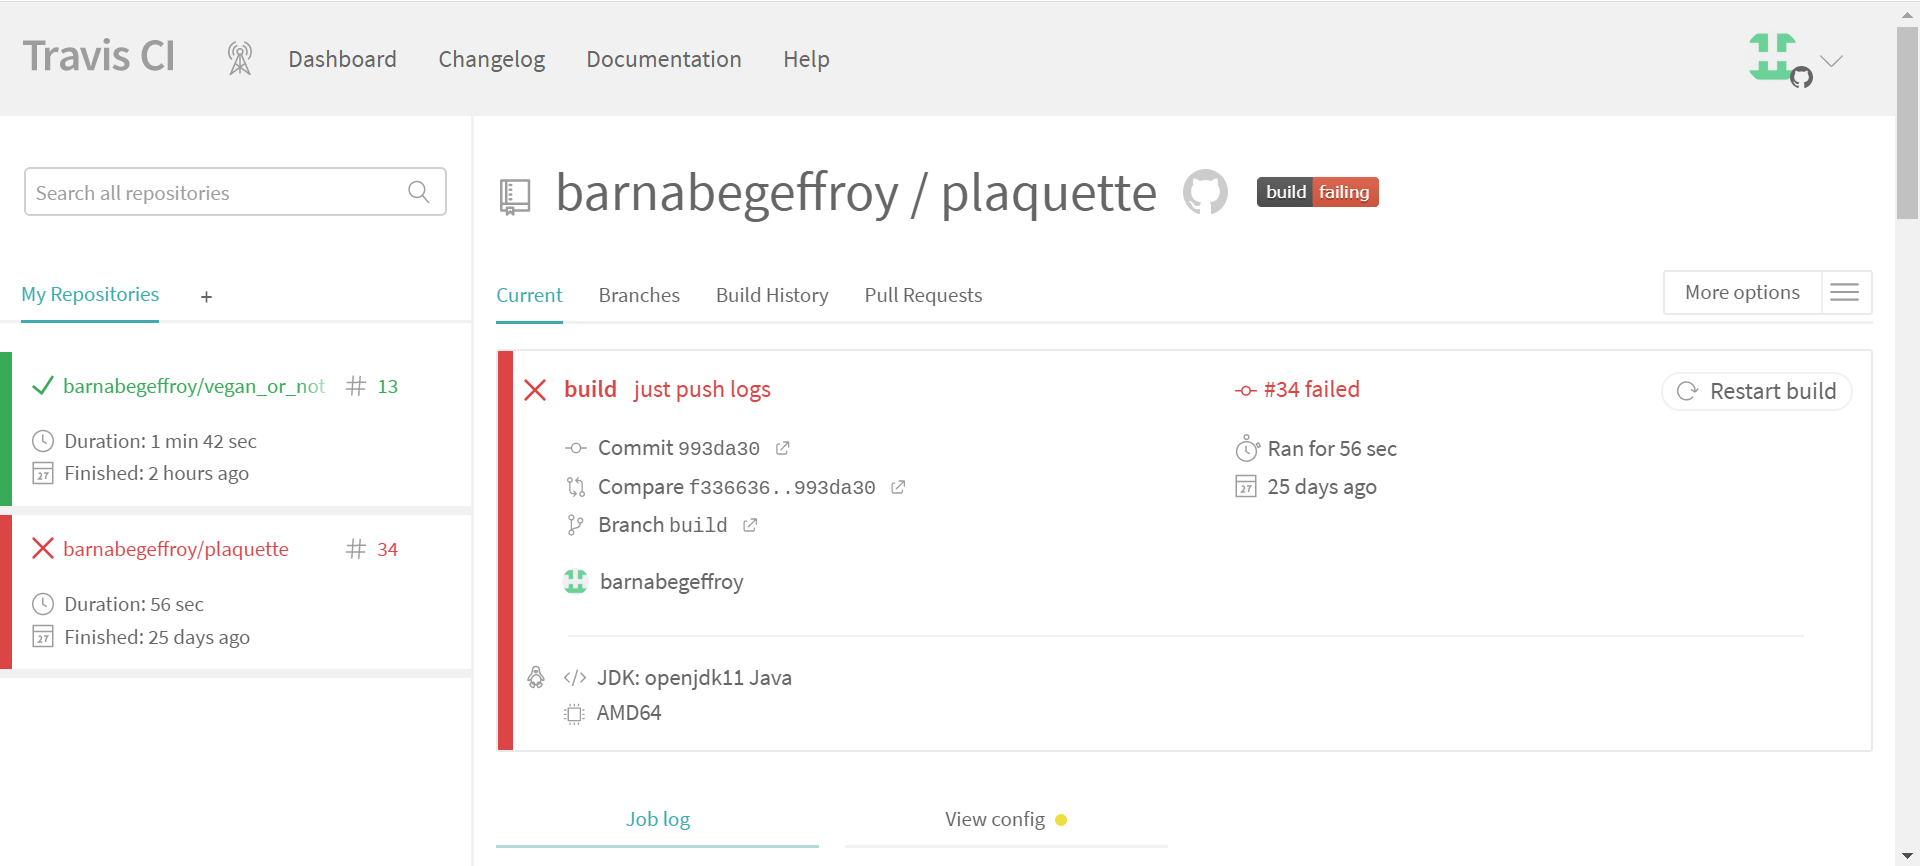
\includegraphics[width=11cm]{assets/travis-ci.PNG}
    \end{center}
    \caption{Capture d'écran de l'interface de Travis-CI}
    \label{travis}
\end{figure}

La figure~\ref{travis} montre que la construction du commit \texttt{just push logs} a échoué pour le dépôt \texttt{plaquette}, tandis que celle du dépôt \texttt{vegan\_or\_not} a réussi.

Travis-CI permet également de référencer des variables d'environnement sécurisées (clefs d'accès, identifiants, ...).
\begin{figure}[!ht]
    \begin{center}
    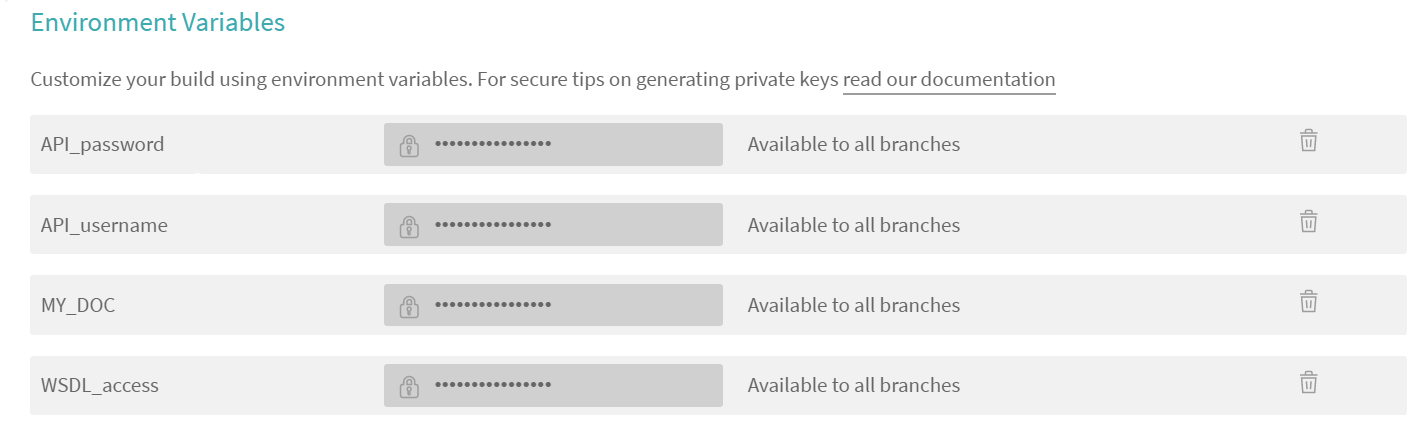
\includegraphics[width=0.8\textwidth]{assets/env.PNG}
    \caption{Différentes variables d'environnement entréees pour la construction Travis-CI d'un dépôt}
    \label{env}
    \end{center}

\end{figure}

\subsection{L'exécution du code}
\subsubsection*{Les dépendances}



Travis-CI identifie automatiquement un projet Maven et installe les dépendances indiquées dans le \texttt{pom.xml}. Dans le projet Plaquette-MIDO, la dépendance qui importe le code source de l'API de Dauphine nécessite un fichier texte nommé \texttt{WSDL\_Login.txt} contenant un URL spécifique aux identifiants de l'utilisateur. Ce fichier ne peut pas être dans le dépôt car il contient des informations personnelles. Il faut un script qui crée le fichier sur la machine virtuelle de Travis-CI. Le fichier doit être créé avant de lancer l'installation des dépendances . Dans le \texttt{.travis.yml}, on peut ajouter un script qui génère ce fichier. 

Voici ci-dessous un extrait de mon implémentation permettant la création d'un tel fichier. On y retrouve les variables d'environnement présentées dans la figure~\ref{env}.

\begin{figure}[!ht]
    \lstinputlisting[language=bash, firstline=18]{./assets/writeWSDL}
    \caption*{Extrait de writeWSDL.sh, annexe~\ref{sec:writeWSDL} }
\end{figure}

\subsubsection*{Création du fichier PDF et déploiement}
Une fois que toutes les dépendances du projet Maven sont installées, il faut executer le code source qui génère le fichier PDF. La classe qui permet cette génération est \texttt{M1ApprBuilder}. Le script de Travis-CI va exécuter cette classe, il faudra ensuite déployer vers un dépôt d'arrivée le fichier PDF ainsi que le logs de la construction. La construction de Travis-CI doit échouer si le fichier PDF n'est pas généré. Néanmoins, dans tous les cas les logs doivent être poussés vers le dépôt. Ainsi, si le fichier PDF est généré, il est poussé avec les logs vers le dépôt d'arrivée. Si ce n'est pas le cas, la construction échoue, le dernier PDF déployé reste disponible. Nous sommmes avertis immédiatement par e-mail de cet échec. Les logs du code source de Plaquette-MIDO ainsi que ceux de Travis-CI permettront alors d'expliquer de l'échec.

Vous trouverez mon implémentation du script exécuté par Travis-CI dans l'annexe~\ref{sec:cibuild}. Le script exécute plusieurs fonctions :

\begin{itemize}
    \item \texttt{clean} (l.20 à 24), supprime les fichiers déjà existants.
    \item \texttt{get\_current\_deploy} (l.26 à 30), copie sur la machine virtuelle de Travis-CI le dépôt dans lequel les fichiers vont être déployés. Pour éviter de cloner un dépôt \texttt{Git} dans un autre dépôt \texttt{Git}, celui-ci est cloné dans le dossier parent de Plaquette-MIDO de la machine virtuelle \texttt{"../\${REPO}"}.
    \item \texttt{build\_doc} (l.31 à 41), essaie de générer le document en exécutant \texttt{M1ApprBuilder}. Elle met aussi à jour la variable \texttt{BUILT\_EXIT\_CODE} qui prend la valeur 0 si le code est correctement exécuté et que le fichier PDF est généré, ou la valeur 1 sinon.
    \item \texttt{deploy} (l.43 à 60), déplace les logs et le fichier PDF (s'il y en a un) vers le dépôt d'arrivée (\texttt{"../\${REPO}"}). Les différentes commandes \texttt{Git} présentées ultérieurement sont alors executées pour déployer les fichiers déplacés.\\ La dernière ligne \texttt{exit \${BUILT\_EXIT\_CODE}} renvoie à Travis-CI la valeur mis à jour dans \texttt{build\_doc}. Si la valeur est 0, la construction contiue et s'achève par un succès. Sinon la construction échoue et une notification est envoyée pour prévenir les développeurs.
\end{itemize}


\subsubsection*{Automatisation}
Travis-CI lance initiallement la construction du code du dépôt à chaque nouveau commit. Il est cependant possible de configurer des \textit{Cron Jobs}. Ceux-ci vont renouveler la construction du code de manière quotidienne, hebdomadaire ou mensuelle. 

\begin{figure}[!ht]
    \begin{center}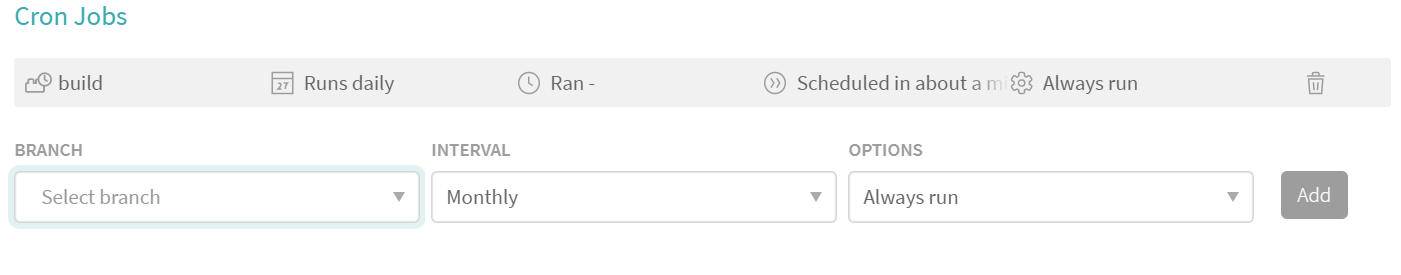
\includegraphics[width=\textwidth]{assets/CronJobs.PNG}
    \end{center}
    \caption{Les \textit{Cron Jobs} de Travis-CI, ici la construction est programmée quotidiennement}
\end{figure}

En programmant sur \textit{Daily}, Travis-CI va relancer la construction du code tous les jours et ainsi renouveller le fichier PDF et les logs si des changements sont effectués. Si une erreur se produit et que le fichier PDF n'est pas généré, une e-mail nous préviendra de la non-construction du code et le fichier PDF le plus récent sera toujours disponible sur le site.

\section{L'authentification}

Pour se connecter à l'API de Dauphine, un nom d'utilisateur et un mot de passe sont nécessaires. Le code initial prévoyait trois manières de fournir ces informations afin de se connecter à l'API :
\begin{itemize}
    \item les propriétés du système
    \item les variables d'environnement
    \item un fichier texte contenant les informations nécessaires
\end{itemize}

Cependant, ce code ne lisait initialement que le mot de passe et le nom d'utilisateur était une valeur par défaut. Un nouvel utilisateur devait modifier le code pour pouvoir utiliser ses identifiants. L'idée d'une valeur par défaut pour le nom d'utilisateur a donc été abandonnée pour rendre le programme plus accessible. La valeur du nom d'utilisateur serait lue de la même manière que celle du mot de passe.

\subsection{La classe Authentication}

Une nouvelle classe, \texttt{Authentication}, a été créée pour permettre la généralisation lecture du code et améliorer sa lisibilité. Celle-ci permet de créer un objet contenant un nom d'utilisateur et un mot de passe de type \texttt{Optional}. Ce type permet d'instancer aussi bien la valeur d'une chaîne de caractère que l'absence d'une information. Cette classe \texttt{Authentication} est lu dans une autre classe, \texttt{QueriesHelper}, qui permet de renvoyer les informations nécessaires pour se connecter à l'API. L'introduction de la classe \texttt{Authentication} permet ainsi de détecter si le nom d'utilisateur ou le mot de passe manquent et alors jeté une exception appropriée faisant échoué l'exécution du code. 

\subsection{Le projet CredsRead}
La généralisation du code permettant l'authentification nous a poussés à séparer dans un projet bien distinct de Plaquette-MIDO, le projet CredsRead. En effet, les méthodes de \texttt{QueriesHelper} ainsi que la classe \texttt{Authentication} n'avait, en grande partie, aucun lien spécifique avec plaquette-MIDO et pouvait ainsi être totalement publiées dans un autre projet pour pouvoir réutiliser plus facilement ce code dans d'autres projets. Le projet Creds-Read a ensuite été intégré au code source de Plaquette-MIDO.